\documentclass{article}
\usepackage[utf8]{inputenc}
\usepackage[margin=3cm]{geometry}
\usepackage{amsmath}
\usepackage{graphicx}
\usepackage{xcolor}
\usepackage[style=authoryear-comp,natbib=true]{biblatex} %Imports biblatex package
\ExecuteBibliographyOptions{bibencoding=utf8,minnames=1,maxnames=2, maxbibnames=99,dashed=false,terseinits=true,giveninits=true,uniquename=false,uniquelist=false,doi=false, isbn=false,url=true,sortcites=false}
\usepackage{appendix}
\usepackage{multirow}

\addbibresource{refs.bib} %Import the bibliography file

\graphicspath{{./figs/}}
\title{Liquidity Forecasting - IMF Working Paper}
\author{Romain Lafarguette and Anastasios Panagiotelis}
\date{May 2022}

\begin{document}
\maketitle

\begin{abstract}
    Forecasts of autonomous liquidity factors are a key input into the operational decisions of central banks. Different methods for forecasting autonomous liquidity factors (currency in circulation, state account balance, net foreign assets and their aggregate) are proposed. Forecasts are evaluated using a data set from the Central Bank of the United Arab Emirates. In an expanding window forecast evaluation, we find models that account for holiday effects, multiple types of seasonality and an asymmetric volatility response and model averaging lead to the best forecast accuracy. Forecast reconciliation improve forecast accuracy for all series, excluding the state account balance.
\end{abstract}

\section{Introduction}

Liquidity management is a key responsibility of central banks to ensure stability of the banking system. Operational decisions rely on accurate forecasts of autonomous liquidity factors. For a discussion of the importance of these forecasts we refer the reader to \citet{Bin2001}, \citet{VeyGuo2019} and references therein. The literature on evaluating different forecasting models for autonomous liquidity factors is rather sparse, perhaps due to the lack of publicly available data at a daily frequency. A notable exception is \citet{CabEtAl2009} who only model currency in circulation using ARIMA and state space models. In this paper we apply a number of contemporary forecasting methods to forecast all autonomous factors as well net liquidity, for the United Arab Emirates (UAE).

{\textit{\color{blue} RF to potentially discuss what is in Section 3 to here instead.}}

Two autonomous factors, namely currency in circulation and state account balance follow distinct seasonal patterns due to calendar effects related to the work week, payment of salaries, public and religious holidays and payment of taxes. These effects make it possible to develop point forecasting models for the level of these factors. On the other hand, net foreign assets do not display seasonal patterns, but do exhibit conditional volatility characteristic of financial returns data. For this reason, in this paper we propose forecasting net foreign assets using models for conditional heteroskedasticity.

In addition to developing forecasting models for three individual autonomous factors we also consider forecast combination through taking an equally weighted combination either of all forecasts or of a trimmed set of models. Finally, we also apply the method of forecast reconciliation to the liquidity forecast problem. This involves first generating forecasts for the aggregate (or net) liquidity due to net foreign assets, currency in circulation and state account balance, leading to four forecasts (one for each autonomous factor and one of the aggregate). In general, these four forecasts will not be coherent, i.e. the aggregate forecast will not be equal to the aggregate of the three individual factors. Reconciliation adjusts the four forecasts to ensure coherence. This method has been shown to improve forecasts in a number of contexts and is applied to liquidity forecasting for the first time here.

The remainder of the paper is summarised as follows. Section~\ref{sec:data} introduces the data on the autonomous factors, highlighting the main features of each factor. Section~\ref{sec:liqman} discussed the operational context of forecasting autonomous liquidity factors in more detail. Section~\ref{sec:data} introduces the models and methods used both for forecasting and forecast reconciliation. Section~\ref{sec:res} presents the results of extensive forecast evaluation and Section~\ref{sec:conc} concludes.

\section{Data}\label{sec:data}

There are several sources of liquidity in a banking system, those that are not under the control of a central bank and therefore represent sources of uncertainty. These are known as \textit{autonomous factors}. The autonomous factors for which forecasting models are built in this study are \textit{currency in circulation}, the \textit{state account balance} and \textit{net foreign assets}. Our data were obtained from the Central Bank of the United Arab Emirates (UAE) and are collected at a daily frequency. We now discuss each of the autonomous factors in turn.

\subsection{Currency in Circulation}

Currency in Circulation (CIC) is the quantity of money issued by monetary authorities net of currency that has been removed from the money supply. 

\textit{\color{blue} RF to potentially expand on CIC data, how collected, measured etc.}

Currency in Circulation tends to be influenced by calendar effects. In many countries, salaries are paid at the same time each week (or month) leading to a smooth weekly (or monthly pattern) whereby CIC increases after the pay date and slowly declines until just before the next pay date. The weekly pattern in CIC can also be influenced by a tendency of individuals to withdraw cash before the weekend. Public holidays can have a major impact on CIC, it is typical for CIC to increase in the buildup to a public holiday and then decline afterwards. These systematic features make it possible to develop models for forecasting CIC at horizons of 1 to 14 days that outperform na\"ive forecasting techniques.

Figure~\ref{fig:cicdata} highlights CIC data for the UAE. Days with missing data include weekends (Friday and Saturday in the UAE) and major holidays. Data on these days are linearly interpolated. Other autonomous factors which may exhibit a different pattern of missingness (for instance data may be available on Fridays for net foreign assets since foreign exchange markets trade on Friday), are interpolated in a similar fashion. As such, interpolating rather than ignoring missing data guarantees a balanced panel of data, which becomes important for reconciliation steps later on. The daily pattern of CIC is apparent from the figure as are spikes around major holidays, in particular Eid al Fitr and Eid al Adha. In early 2020 there is a permanent level shift in CIC associated with measures at the onset of Covid to inject cash into the monetary system.

\begin{figure}[!h]
    \centering
    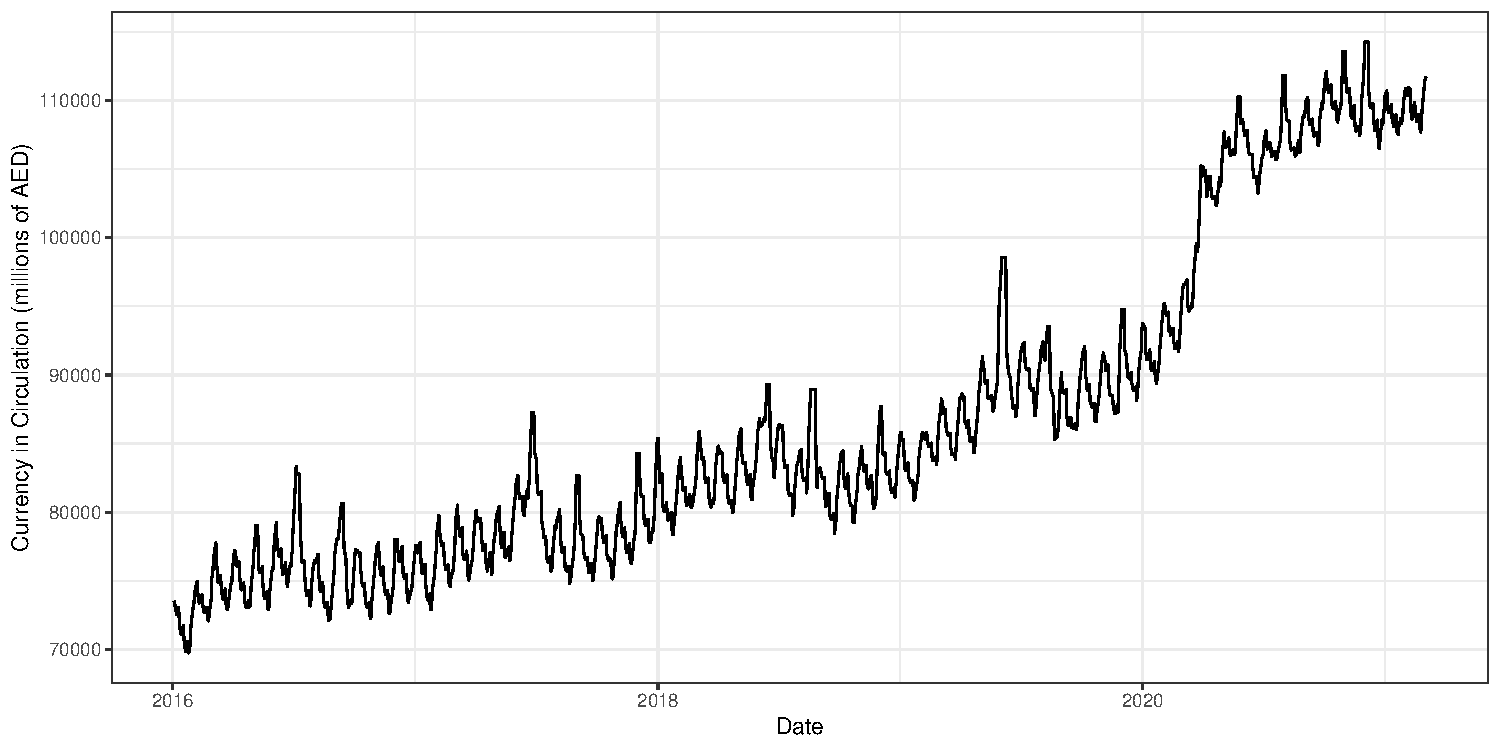
\includegraphics[scale=0.6]{cicplot}
    \caption{Currency in Circulation data for the United Arab Emirates measured in million of Dirhams.}
    \label{fig:cicdata}
\end{figure}

\subsection{State Account Balance}

State Account Balance (SAB) is the quantity of money held by the government in its account with the Central Bank. 

\textit{\color{blue} RF to potentially expand on SAB data, how collected, measured etc.}

State Account Balance also tends to be influenced by calendar effects. In particular certain taxes may be due for collection towards the end of the week, month, quarter of financial year which can provide a boost to SAB at these time. Models accounting for these features can also outperform na\"ive approaches in forecasting SAB. 

Figure~\ref{fig:sabdata} highlights SAB data for the UAE. Apart from spikes associated with seasonal factors, there is also a large one off spike in early 2019 associate with the sale of government assets. In our modelling, such transitory effects can be accounted for via the use of dummy variables. When asset sales are scheduled to occur at some time in the future, this may motivate judgemental adjustments to model forecasts.

\begin{figure}[!h]
    \centering
    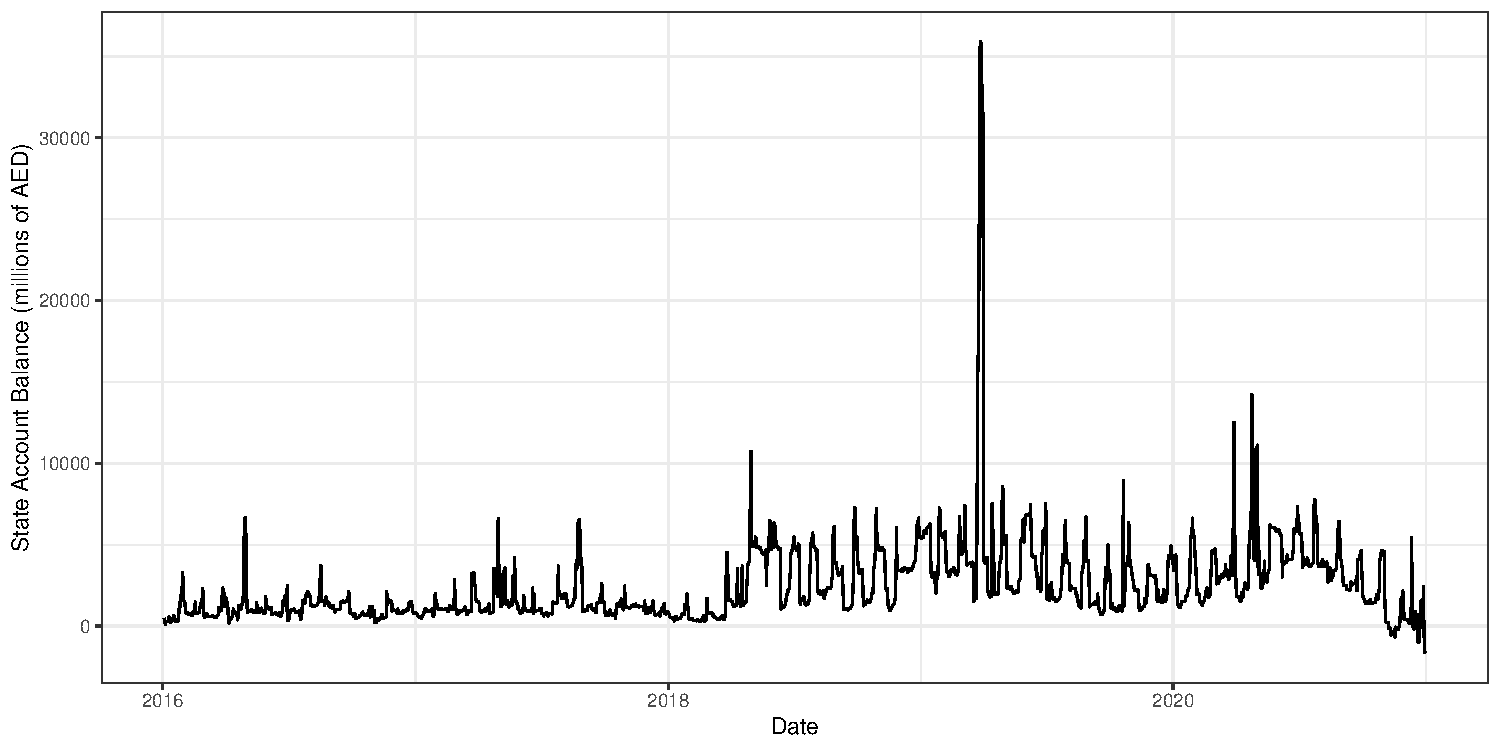
\includegraphics[scale=0.6]{sabplot}
    \caption{State Account Balance data for the United Arab Emirates measured in million of Dirhams.}
    \label{fig:sabdata}
\end{figure}

\subsection{Net Foreign Assets}

Net Foreign Assets (NFA) is the total foreign assets held by a central bank, net of their foreign liabilities

\textit{\color{blue} RF to potentially expand on NFA data, how collected, measured etc.}

Compared to other autonomous factors, NFA are not influenced by calendar effects and when forecasting the mean, it is often difficult to outperform a na\"ive forecast of last observed value of NFA. However the daily change in NFA do resemble financial returns in that they often exhibit conditional heteroskedasticity and volatility clustering. This makes the GARCH family of models good candidates for forecasting the entire distribution of NFA data, which can be a critical input into operational decisions of Central Banks in the money market.

Figure~\ref{fig:nfadata} shows both the level (top panel) and change (bottom panel) in net foreign assets. The bottom panel in particular shows evidence of conditional heteroskedasticity motivating the use of GARCH models and their extensions

\begin{figure}[!h]
    \centering
    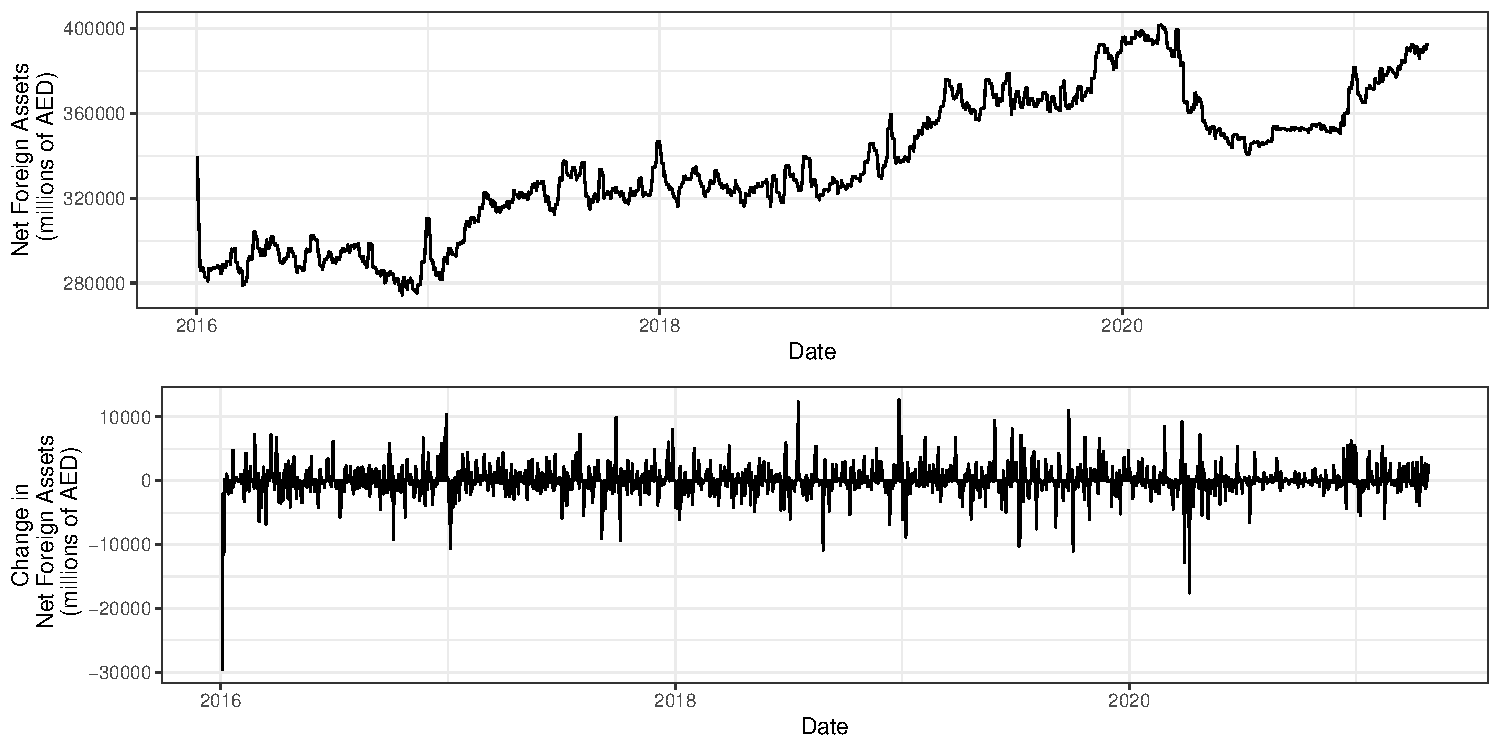
\includegraphics[scale=0.6]{nfaplot}
    \caption{Net Foreign Assets data for the United Arab Emirates measured in million of Dirhams. Top panel: level, bottom panel: change.}
    \label{fig:nfadata}
\end{figure}

\subsection{Aggregate}

The aggregate (AGG) for the autonomous factors (or net liquidity due to autonomous factors) is given by 

\[
AGG=NFA-(CIC+SAB)
\]

This reflects the fact that while NFA are clearly assets on the central bank balance sheet, CIC and SAB are liabilities for a central bank. This aggregate represents the net liquidity due to autonomous factors. While this aggregate is composed of all autonomous factors, in general the scale of NFA is much higher than CIC and SAB. As a result, the high variability of NFA tends to dominate this time series. Suitable models for forecasting the aggregate series are thus models for conditional volatility. However, information from CIC and SAB can be incorporated into the forecast of the aggregate via forecast reconciliation methodology, discussed in more detail in Section~\ref{sec:forereco}.

Figure~\ref{fig:aggdata} shows the net liquidity due to autonomous factors for the UAE. The top panel shows the level, the bottom panel shows the change. It is clear that variability of the NFA data dominates the influence of CIC and SAB. While the predictable seasonal patterns of CIC and SAB should in principle help with forecasting the aggregate, it will be difficult to model these effects while modelling the aggregate series alone. Later, this motivates forecast reconciliation approaches where separate models are developed for each of the autonomous factors and the aggregate.

\begin{figure}[!h]
    \centering
    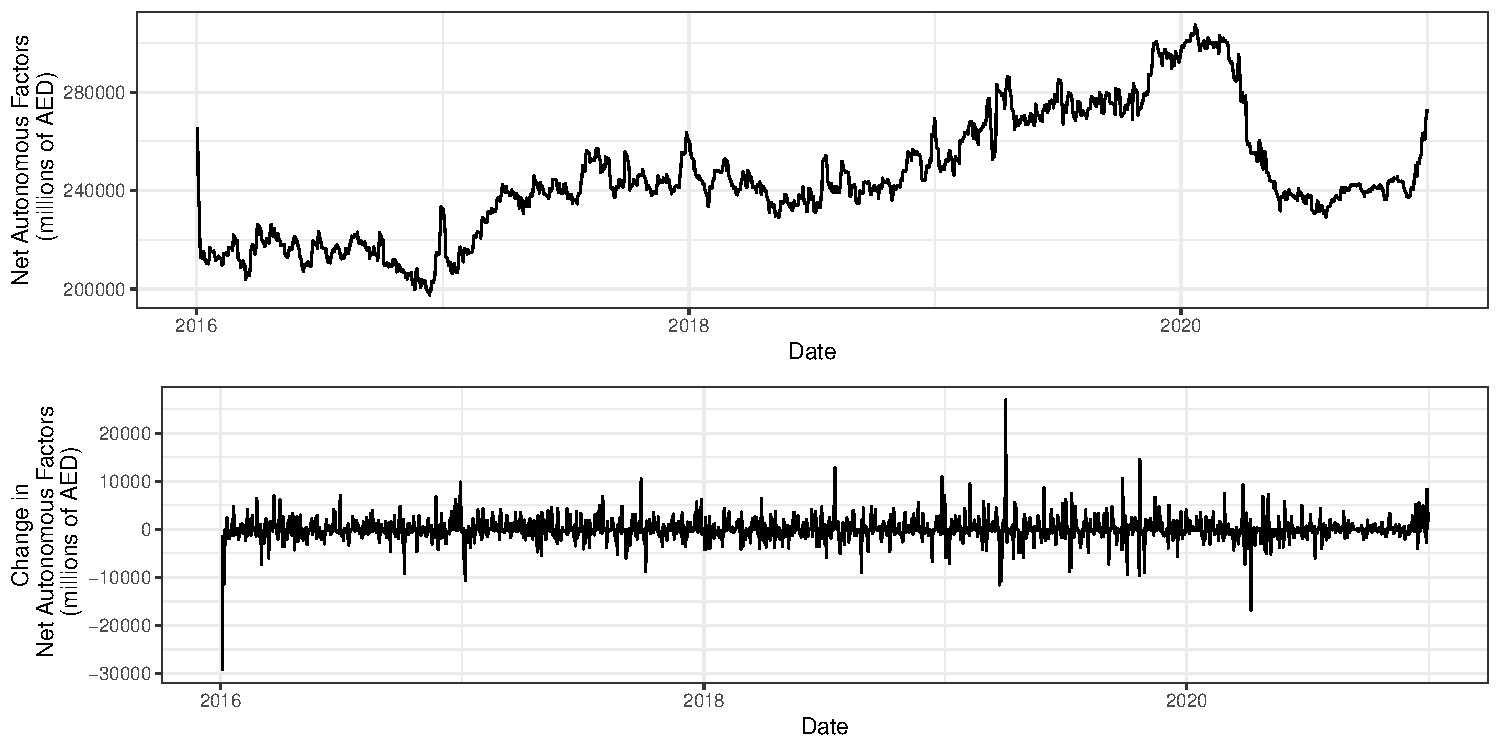
\includegraphics[scale=0.6]{aggplot}
    \caption{Net liquidity due to autonomous factors for the United Arab Emirates measured in million of Dirhams. Top panel: level, bottom panel: change.}
    \label{fig:aggdata}
\end{figure}

\section{Liquidity Management}\label{sec:liqman}

{\color{blue}
\textit{RL to contribute. Discuss:}


\textit{\begin{itemize}
    \item Context of the Forecasting Problem
    \item Importance of getting probabilistic forecasts 
    \item etc...
\end{itemize}}

Alternatively, this discussion could be in the introduction.

}

\section{Models}\label{sec:models}

We now give a brief description to modelling approaches that can be used for forecasting autonomous factors. As a reference to the general model classes described below see \cite{HynAth2021} and (for conditional volatility models) \citet{Tsay2005}. Throughout, $y_t$ denotes the value of an autonomous factor at time $t$, $\hat{y}_{t+h}$ denotes the $h$ day ahead forecast of an autonomous factor, made at time $t$, $m$ denotes the seasonal period (in our context $m=7$ for each day of the week) and $k$ is the integer part of $(h-1)/m$

%\subsection{Na\"ive Forecasts}

%The naive forecast is given by the last available value of the time series i.e $\hat{y}_{t+h}^{Naive}=y_{t}$. Alternatively for series with a weekly pattern (such as CIC) the last value available observed on the same day of the week of the previous period i.e., $\hat{y}_{t+h}^{SNaive}=y_{t+h-m(k+1)}$

\subsection{Exponential Smoothing}

ETS models are a class of models that employ exponential smoothing with trend and seasonal components \citep[see][for details]{HynEtAl2008}. The level, trend and seasonal components at time $t$ are given by $l_t$, $b_t$ and $s_t$ respectively. Equations for forecasts and for updating the components are given by

\begin{align}
\hat{y}_{t+h}&=l_t+hb_t+s_{t+h-m(k+1)}\\
l_t&=\alpha (y_t-s_{t-m})+(1-\alpha)(l_{t-1}+{b_{t-1}})\\
b_t&=\beta (l_t-l_{t-1})+(1-\beta)b_{t-1}\\
s_t&=\gamma (y_t-l_{t-1}-b_{t-1})+(1-\gamma)s_{t-1}\,,
\end{align}

where $\alpha$, $\beta$ and $\gamma$ are parameters that control the smoothness of the level, trend and seasonal components respectively that can be estimated by maximum likelihood. The model can be extended to allow for  multiplicative trends (with or without damping) seasonal components, and errors. Depending on the components included and whether they are additive or multiplicative, leads to 30 possible model specifications. All specifications are fit and the model with the lowest corrected Akaike Information Critrion (AICc) given by

$$-2lnL+\frac{2q(q+1)}{T-q-1}$$

where $q$  is the number of model parameters and $T$ is the size of the training sample, is chosen. The \texttt{ets} function in the \texttt{forecast} package \citep{ForPac} in the R programming environment \citep{R2020}.

\subsection{ARIMA}

The ARIMA class of models take the form

\[(1-\phi(L))(1-L)^d(y_t-\mu)=(1+\theta(L))\epsilon_t\]

where $d$ is the degree of differencing, $L$ is the lag operator, $\phi(L)=\phi_1L+\phi_2L^2+\dots+\phi_pL^p$ is a lag polynomial of AR parameters and $\theta(L)=\theta_1L+\theta_2L^2+\dots+\theta_qL^q$ is a lag polynomial of MA parameters.

The auto arima algorithm \citep{HynKha2008} can be used to select to orders $p$, $q$ and $d$. First the degree of differencing $d$ is determined by the sequqntial application of the KPSS test for stationarity. Then using the differenced data, an AR(1), AR(2) and ARMA(2,2) are fit. Starting from the model that minimises AICc, a search amongst neighboring models (i.e. models with $p$ or $q$ that differ by one from the current best model) is used to determing $p$ ad $q$.

For seasonal data, a seasonal ARIMA

\[(1-\phi(L))(1-\Phi(L^m))(1-L)^d(1-L^m)^D(y_t-\mu)=(1+\theta(L))(1-\Theta(L^m))\epsilon_t
\]

can be used instead, where $P$, $D$ and $Q$ are the orders of the seasonal AR polynomial, differencing and MA polynomial respectively. The auto arima algorithm can be modified to account for seasonality. This is implemented by the \texttt{auto.arima} function of the \texttt{forecast} package

\subsection{ARIMA with regression}

To capture the effects of holidays as well as longer seasonal patterns (e.g. yearly patterns) ARIMA models can be combined with regression. In particular, regression models are fit (possibly after differencing) with the errors then assumed to follow an ARMA process. The following regressors are considered in our modelling framework

\subsubsection{Day of Week Dummies}

Dummy variables can be used to capture weekly patterns in the data. This is particularly well suited to cases where the weekly pattern remains the same over the entire time series. It is less well suited when the seasonality varies over time, in which case seasonal ARIMA models may be more appropriate.

\subsubsection{Fourier Terms}

To capture smooth effects that take place over a longer seasonal period, Fourier terms can be used. These come in pairs and take the form
\[
x_{j,t}^{(c)}=\cos(2\pi jt/m)\textrm{  and  } x_{j,t}^{(s)}=\sin(2\pi jt/m)
\]

for $j=1,\dots,J$ and where $m$ is a longer seasonal period such as $m=365$ (days in the year). For countries with a majority Muslim population $m=354$ can be used to capture the effect of religious events (e.g. Ramadan) as well as religious holidays (e.g. Eid al Adha, Eid al Fitr) that move relative to the Gregorian calendar. In the case of the UAE, we construct Fourier terms based on four seasonal periods, $m=30$ roughly corresponding to monthly effects, $m=90$ roughly corresponding to quarterly effects, and $m=354$ and $m=365$ corresponding to the religious and civic year respectively.

\subsubsection{Holiday effects}

A standard approach to modelling the effects of holidays is to use dummy variables, which would capture a spike in an autonomous factor on a holiday. However, in the case of forecasting CIC in particular, what is more commonly observed is a ramping up of CIC for a week before a holiday, before a ramping down of CIC for a week after the holiday. This is captured by constructing the following covariate

\[
x_t^{(h)}=\max\left(\underset{t^*\in\mathcal{T}_{hol}}{\max}\left(\frac{t^*-t}{7}\right)^2,0\right)
\]

where $\mathcal{T}_{hol}$ is a set of all $t$ such that day $t$ is a public holiday. If there is a public holiday within 7 days of day $t$, the term $t^*-t$ measures the amount of days before/after a holiday. This creates a small quadratic hump around each holiday (and bears some similarities with the Prophet model \citep{TayLet2018} which uses a Gaussian density). For days that do not occur within a week of a public holiday $x_t^{(h)}=0$.

\subsubsection{Structural Breaks}

Two forms of structural breaks are often observed in autonomous factors. A transitory structural break sees a change in the level of a series for a short period. In this case dummies can be used equal to 1 for the duration of the transitory structural break and 0 otherwise. This is implemented in the case of the State Account Balance for the UAE, with a transitory break starting on March 23, 2020 and ending on April 1, 2020. Alternatively there are permanent structural breaks which see a sustained change in the level of an autonomous factor. These are modelled using dummy variables set to zero before the structural break and one after the structural break. In the case of the UAE, this was implemented for the CIC data from the March 17, 2020.

\subsubsection{Predictor Selection in Regression}

Since only a small number of groups of regressors are considered, covariates can be chosen by an exhaustive search. To clarify, blocks of day of week dummies, Fourier terms (for each seasonal frequency), holiday dummies and structural break dummies, are either included or excluded all at once, leading to $2^4=16$ model specifications. For each both non-seasonal and seasonal ARIMA errors are considered with the auto arima algorithm used to select the ARIMA orders. The model with the lowest AIC overall is then selected. An alternative to this approach would be to carry out a LASSO to conduct variable selection, or, if the blocked structure of predictors is to be preserved, then a blocked LASSO can be used instead. An advantage of an exhaustive search is that it allows the regression specification and ARIMA specification for the errors to be chosen simultaneously - although it should be noted that an exhaustive search can be computationally demanding.

\subsection{TBATS}

The TBATS model \citep{DeLEtAl2011} is a form of exponential smoothing model with a number of additional features. Seasonality evolves according to Fourier terms (similar to those used in the regression model), the series is transformed by a Box-Cox transformation (which includes the log transformation as a limiting case) and the errors of the model follow an ARMA model. The main advantage of this model is that multiple seasonal components can be used accounting for seasonality with different periodicities. This is particularly useful in countries where civic and religious calendars may differ for example, in countries with a majority Muslim population. For the UAE, TBATS is implemented with seasonal periods of $m=7,30,90,354,365$, roughly corresponding to days in a week, month, quarter, religious year and civic year.

\subsection{Conditional Heteroskedasticity models}

Net foreign assets and the aggregate series tend to resemble series on asset prices, with conditional heteroskedasticity in the difference of these series a major feature. To capture this we consider models in the GARCH family of distributions. All models for conditional volaitlity were implemented using the \texttt{rugarch} package in R~\citep{rugpac}. The standard GARCH specification \citep{Bol1986} is given by

\begin{align}
  u_t&=\sigma_t\epsilon_t\\
  \sigma_t^2&=\omega+\alpha_1u^2_{t-1}+\dots+\alpha_pu^2_{t-p}+\beta_1\sigma^2_{t-1}+\dots+\beta_q\sigma^2_{t-q}
\end{align}

where $u_t$ are demeaned changes in net foreign assets and $\epsilon_t$ is white noise with zero mean and unit variance. In modelling NFA, we consider a GARCH(1,1) specification where $p=q=1$. This model is estimated by (quasi-)maximum likelihood under the assumption that $\epsilon_t$ is normally distributed. Both stationarity and enforcing that variances are positive impose certain constraints on these parameters.

An special case of the GARCH(1,1) model that is non-stationary in given by the EWMA process 

\begin{align}
  u_t&=\sigma_t\epsilon_t\\
  \sigma_t^2&=\lambda u^2_{t-1}(1-\lambda)\sigma^2_{t-1}
\end{align}

which is a form of simple exponential smoothing for the variance rather than the mean process. An extension of the GARCH(1,1) model is the GJR-GARCH(1,1) model \citep{GloEtAl1993}

\begin{align}
  u_t&=\sigma_t\epsilon_t\\
  \sigma_t^2&=\omega+\alpha u^2_{t-1}+\gamma I(u_t>0)u^2_{t-1}\beta\sigma^2_{t-1}
\end{align}

The rationale behind the GJR-GARCH model is that the response of volatility will be stronger following a negative change in the variable rather than a positive change.

The final model we consider for conditional heteroskedasticity is the EGARCH(1,1) model \cite{Nel1991} given by

\begin{align}
  u_t&=\sigma_t\epsilon_t\\
  \ln(\sigma_t^2)&=\omega+\alpha \left(|\epsilon_{t-1}|+\gamma\epsilon_{t-1}\right)+\beta\ln(\sigma^2_{t-1})
\end{align}

An advantage of the EGARCH model is that the parameters do not need to be constrained in a way that ensures positive variances since all modelling of the variance takes place on the log scale. 

\subsection{Model Averaging}

It is well established in the forecasting literature that combining forecasts from different classes of models can improve forecast accuracy~\citep{Tim2006}. While there is a long literature on finding optimal weights, even weights tend to perform more robustly since there is no additional uncertainty introduced by having to estimate combination weights~\citep{SmiWal2009}. As well as considering an equally weighted combination of all classes of models outlined above, we also consider trimming models by only taking the best $K$ models. For this studey we consider $K=2$.%Trimming can also be achieved using model confidence sets \citep{SamSek2017} so that all models not found to perform significantly worse that the best model are used to combine forecasts.

\subsection{Forecast Reconciliation}\label{sec:forereco}

When forecasts are generated for the autonomous factors (CIC, SAB and NFA) as well as AGG, there is no guarantee that forecasts respect the aggregation relationship $AGG=NFA-(CIC+SAB)$. To address this issue, different approaches can be used. As a benchmark, consider the case of ignoring that forecasts do not aggregate correctly, this is known as a 'base' or unreconciled forecast. In the following it is convenient to stack these base forecasts in a vector

\[
\hat{\boldmath{y}}_t=\begin{pmatrix}\hat{\textrm{AGG}}_t\\
\hat{\textrm{CIC}}_t\\
\hat{\textrm{SAB}}_t\\
\hat{\textrm{NFA}}_t\end{pmatrix}
\]

The first approach to achieve coherent forecasts is to ignore the base forecast of the aggregate and instead simply compute an aggreagate forecast as 
$\hat{\textrm{NFA}}_t-(\hat{\textrm{CIC}}_t+\hat{\textrm{SAB}}_t)$. This is known as a bottom up approach. A more modern approach that does uses forecasts at all levels is forecast reconciliation.

Reconciliation methods require defining a matrix which in the case of autonomous factors is given by

\[
\mathbf{S}=\begin{pmatrix} -1 & -1 & 1\\
1 & 0 & 0\\
0 & 1 & 0\\
0 & 0 & 1\\
\end{pmatrix}
\]

The first row of this matrix encodes the relationship between net liquidity and the autonomous factors. The second approach to obtain coherent forecasts is the so called OLS method of reconciliation \citep{HynEtAl2011} given by

\[
\tilde{\mathbf{y}}=\mathbf{S}\left(\mathbf{S}'\mathbf{S}\right)^{-1}\mathbf{S}'\hat{\mathbf{y}}
\]

By construction the reconciled forecasts $\tilde{\mathbf{y}}$ will cohere to the aggregation constraint.

The third way used to obtain coherent forecasts is an improvement on OLS reconciliation, known as the Minimum Trace (MinT) method\citep{WicEtAl2019}.  This method accounts for covariance in the forecasting errors of each autonomous factor. Reconciled forecasts using the the MinT method are given by

\[
\tilde{\mathbf{y}}=\mathbf{S}\left(\mathbf{S}'\boldsymbol{\Sigma}^{-1}\mathbf{S}\right)^{-1}\mathbf{S}'\boldsymbol{\Sigma}^{-1}\hat{\mathbf{y}}
\]

The covariance matrix $\boldsymbol{\Sigma}$ is estimated using the residuals from the models for each autonomous factor.

\section{Forecast Evaluation}\label{sec:eval}

Forecast evaluation is carried out via an expanding window analysis. All data begin on January 3, 2016. For the first evaluation, all models are trained using available data up to and including data on July 3, 2018. One-step to 14-step ahead forecasts are then produced, i.e. from July 4, 2018 to July 17, 2018. The second evaluation rolls the window one week ahead, i.e. using all data up to and including data on July 10, 2018, forecasts for July 11,2018 to July 24, 2018 are produced. The window is expanded one week at a time up to an origin date of December 15, 2020. This gives a total of 129 origin dates (which we denote $\mathcal{T}_{\textrm{eval}}$, with 14 forecasts at each origin date. The origin dates are all on a Tuesday - a date influence by the operational context in which the Central Bank of the UAE operates.

The $h$-step ahead forecast made at origin date $t$ are denoted $\hat{y}_{t+h|t}$. These are evaluated using RMSE and MAE given by

\[
\textrm{RMSE}_h=\sqrt{\frac{1}{|\mathcal{T}|}\sum_\mathcal{T}(y_t-\hat{y}_{t+h|t})^2}\,\textrm{and}\,\textrm{MAE}_h=\sqrt{\frac{1}{|\mathcal{T}|}\sum_\mathcal{T}|y_t-\hat{y}_{t+h|t}|}
\]

respectively. As a summary measure of forecasting performance over all horizons, squared and absolute errors can be averaged across forecasting horizons as well as forecast origins.

Given the importance of probabilistic forecasting in liquidity management we also require forecast accuracy metrics for probabilistic forecasts. A $100\times\alpha$\% prediction intervals $(\hat{l}_{t+h|t},\hat{u}_{t+h|t})$ can be evaluated by computing the coverage, that is the proportion of times the realised value of a series is does not land within the prediction interval, over the evaluation windows. 

To examine whether the differences in forecasting accuracy between different methods are statistically significant we employ the model confidence set of \citet{HanEtAl2011}. This can be interpreted in a similar fashion to a confidence interval, in the same way that a confidence interval will cover the true value of a parameter with a given probability, the model confidence set will cover the best forecasting model with a given level of probability. The model confidence sets are found using the \texttt{MCS} package in R~\citep{MCSpac} with the default settings of a 15\% Level of Signficance and 5000 bootstrap replications.

%Another way to measure the forecast accuracy of prediction intervals is the Winkler score \citep{Win1972} given by

%\[
%W^{(\alpha)}_{t+h|t}=\left\{
%\arraycolsep=1.4pt\def\arraystretch{2.2}
%\begin{array}{ll}
%\hat{u}_{t+h|t}-\hat{l}_{t+h|t}+\frac{2}{\alpha}(\hat{l}_{t+h|t}-y_{t+h})&\textrm{ if }y_{t+h}<\hat{l}_{t+h|t}\\
%\hat{u}_{t+h|t}-\hat{l}_{t+h|t}&\textrm{ if }\hat{l}_{t+h|t}\leq y_{t+h}\leq\hat{u}_{t+h|t}\\
%\hat{u}_{t+h|t}-\hat{l}_{t+h|t}+\frac{2}{\alpha}(y_{t+h|t}%-\hat{u}_{t+h})&\textrm{ if }y_{t+h}>\hat{u}_{t+h|t}
%\end{array}\right.
%\]

%These can be averaged over the evaluation windows, or over the different forecast horizons to get an overall measure of the accuracy of interval forecasts.

\section{Results}\label{sec:res}

Table~\ref{tab:cicsum} shows MAE of currency in circulation for 1-day ahead, 7-day ahead and 14-day ahead forecasts. At a 1-day horizon and 7-day horizon, the best performing methods are the model averages, however, the differences between models are quite small - the model confidence set contains all models. However at a 14-day horizon, the best performing model is the ARIMA with regression. Only this model, and the model average of the two best models are included in the model confidence set. This indicates the importance of modelling seasonality and events allowed in the regression model with ARIMA errors, especially at a two week horizon.

% latex table generated in R 4.0.3 by xtable 1.8-4 package
% Sun May 29 14:13:46 2022
\begin{table}[!ht]
\centering
\begin{tabular}{lrrr}
  \hline
Method & h=1 & h=7 & h=14 \\ 
  \hline
SES & 379 & 2121 & 3234 \\ 
  ETS & \textbf{363} & \textbf{2098} & 3188 \\ 
  ARIMA & \textbf{359} & \textbf{2012} & 2813 \\ 
  SARIMA & \textbf{378} & \textbf{2223} & 3891 \\ 
  SARIMA Reg. & \textbf{389} & \textbf{1890} & \textbf{2579} \\ 
  TBATS & \textbf{355} & \textbf{2039} & 2786 \\ 
  MA-all & \textbf{340} & \textbf{1865} & 2809 \\ 
  MA-best2 & \textbf{346} & \textbf{1854} & \textbf{2537} \\ 
   \hline
\end{tabular}
\caption{MAE at different forecast horizons (h) for currency in circulation. The methods are Simple Exponential Smoothing (SES), ETS, ARIMA, Seasonal ARIMA (SARIMA), a seasonal ARIMA with regressors for events and trigonometric seasonality (SARIMA Reg.), and two model averages, one an equally weighted average of all models (MA-all), and the other a equally weighted average of the best 2 models (MA-best2). Entries in \textbf{bold} indicate all models in the model confidence set.} 
\label{tab:cicsum}
\end{table}

Table~\ref{tab:sabsum} shows the results for State Account Balance. For this data the ARIMA models, including ARIMA with regression perform poorly at a 1-day horizon with TBATS and a model average performing best, and exponential smoothing methods within the model confidence set. At longer horizons the TBATS model performs well, although it should be noted that at a 7-day and 14-day horizon, it is difficult to distringuish between models with only simple exponential smoothing excluded from the model confidence set.

\begin{table}[!ht]
\centering
\begin{tabular}{lrrr}
  \hline
Method & h=1 & h=7 & h=14 \\ 
  \hline
Simple Exponential Smoothing & \textbf{667} & 1725 & 2010 \\ 
  ETS & \textbf{687} & \textbf{1743} & \textbf{2059} \\ 
  ARIMA & 814 & \textbf{1766} & \textbf{2025} \\ 
  Seasonal ARIMA & 803 & \textbf{1862} & \textbf{1961} \\ 
  SARIMA trig events & 829 & \textbf{1652} & \textbf{1807} \\ 
  TBATS & \textbf{731} & \textbf{1553} & \textbf{1724 }\\ 
  Model Average (all models) & \textbf{728} & \textbf{1604} & \textbf{1845} \\ 
  Model Average (best 2) & \textbf{684} & \textbf{1567} & \textbf{1801} \\ 
   \hline
\end{tabular}
\caption{MAE at different forecast horizons (h) for state account balance. The methods are Simple Exponential Smoothing (SES), ETS, ARIMA, Seasonal ARIMA (SARIMA), a seasonal ARIMA with regressors for events and trigonometric seasonality (SARIMA Reg.), and two model averages, one an equally weighted average of all models (MA-all), and the other a equally weighted average of the best 2 models (MA-best2). Entries in \textbf{bold} indicate all models in the model confidence set.} 
\label{tab:sabsum}
\end{table}

Regarding Net Foreign Assets and net liquidity due to autonomous factors, conditional volatility is the dominant feature of these series. Therefore it makes more sense to report the coverage of 95\% prediction intervals for these series. Table~\ref{tab:nfasum} reports these for net foreign assets. All models achieve coverage close to the desired rate of 95\%, with a GARCH model and an model average performing slightly better than the alternatives across all forecast horizons. Table~\ref{tab:aggsum} shows the same results for net liquidity due to autonomous factors. Again, all models achieve coverage rates close to 95\% with the model averages performing relatively well. It should be noted testing for significant differences in coverage rates will lack power due to the small number of evaluation periods in this empirical study.

\begin{table}[!ht]
\centering
\begin{tabular}{lrrr}
  \hline
Method & h=1 & h=7 & h=14 \\ 
  \hline
EWMA & 0.9250 & 0.9250 & 0.9083 \\ 
  GARCH & \textbf{0.9500} & \textbf{0.9417} & \textbf{0.9333} \\ 
  GJR-GARCH & \textbf{0.9500} & 0.9333 & 0.\textbf{9333} \\ 
  E-GARCH & 0.9333 & \textbf{0.9417} & \textbf{0.9333} \\ 
  MA-all & \textbf{0.9583} & \textbf{0.9417} & \textbf{0.9333} \\ 
  MA-best2 & 0.9333 & 0.9333 & 0.9167 \\ 
   \hline
\end{tabular}
\caption{Coverage of 95\% prediction intervals at different forecast horizons (h) for net foreign assets. The methods are Exponentially Weighted Moving Average (EWMA), GARCH, GJR-GARCH, E-GARCH (SES), and two model averages, one an equally weighted average of all models (MA-all), and the other a equally weighted average of the best 2 models (MA-best2). Entries in \textbf{bold} are those closest to 0.95.} \label{tab:nfasum}
\end{table}

\begin{table}[!ht]
\centering
\begin{tabular}{lrrr}
  \hline
Method & h=1 & h=7 & h=14 \\ 
  \hline
EWMA & 0.9302 & 0.9380 & 0.9302 \\ 
  GARCH & 0.9302 & \textbf{0.9535} & 0.9457 \\ 
  GJR-GARCH & \textbf{0.9380 }& \textbf{0.9535} & 0.9457 \\ 
  E-GARCH & 0.9147 & 0.9612 & 0.9380 \\ 
  MA-all &\textbf{ 0.9380} & 0.9612 & 0.9380 \\ 
  MA-best2 & \textbf{0.9380} & 0.9612 & \textbf{0.9535} \\ 
   \hline
\end{tabular}
\caption{Coverage of 95\% prediction intervals at different forecast horizons (h) for net liquidity due to autonomous factors. The methods are Exponentially Weighted Moving Average (EWMA), GARCH, GJR-GARCH, E-GARCH (SES), and two model averages, one an equally weighted average of all models (MA-all), and the other a equally weighted average of the best 2 models (MA-best2). Entries in \textbf{bold} are those closest to 0.95.} \label{tab:aggsum}
\end{table}

In addition to the forecasts from individual models, we also consider forecast reconciliation methods discussed in Section~\ref{sec:forereco}. For this evaluation we consider the regression model with ARMA errors for CIC, Simple Exponential Smoothing for SAB, an e-GARCH model for NFA and a GJR-GARCH model for AGG. Table~\ref{tab:reco} summarises the mean absolute errors for each series. The results are quite mixed, reconciliation does not guarantee an improvement in forecast accuracy for all factors at all horizons. However, there are instances where reconciliation methods lead to improved forecast accuracy. The forecast of the aggregate improves at a short horizon using the MinT method, and at a long horizon using OLS. The currency in circulation forecast can be improved at a short horizon using OLS reconciliation. Net foreign asset forecasts improve across all horizons using the OLS method. In the meantime the state account balance forecasts are not improved by using reconciliation. This result is consistent with theoretical evidence that while reconciliation can improve forecasting accuracy overall, these improvements are not guaranteed to occur for all series~\citep{PanEtAl2021}. Nonetheless, reconciliation does improve forecasts for some series/ forecasting horizons and most importantly ensures that forecasts are coherent, that is they respect the constraint AGG=NFA-(CIC+SAB).

\begin{table}[ht]
\centering
\begin{tabular}{l|l|rrr}
  \hline\hline
Autonomous Factor & Method & MAE (h=1) & MAE (h=7) & MAE (h=14) \\ 
  \hline
\multirow{4}{*}{Net Liquidity}&Base (Unreconciled) & 1760.32 & \textbf{4301.35} & 5724.03 \\ 
 & Bottom Up & 1807.91 & 4451.54 & 5902.34 \\ 
 & MinT & \textbf{1753.49} & 4397.29 & 5767.77 \\ 
  &OLS & 1768.10 & 4306.73 & \textbf{5715.94} \\ 
  \hline
\multirow{4}{*}{Currency in Circulation}  &Base (Unreconciled) & 377.69 & \textbf{1878.46} &\textbf{ 2567.23} \\ 
  &Bottom Up & 377.69 & \textbf{1878.46} & \textbf{2567.23 }\\ 
  &MinT & 375.61 & 1890.23 & 2583.85 \\ 
  &OLS & \textbf{368.58} & 1889.95 & 2584.56 \\ 
  \hline
\multirow{4}{*}{Net Foreign Assets}  &Base (Unreconciled) & 1423.02 & 4092.57 & 5643.08 \\ 
  &Bottom Up & 1423.02 & 4092.57 & 5643.08 \\ 
  &MinT & 1441.80 & 4131.70 & 5596.20 \\ 
  &OLS & \textbf{1404.91} & \textbf{3976.77} & \textbf{5500.73} \\ 
  \hline
\multirow{4}{*}{State Account Balance}  &Base (Unreconciled) & \textbf{666.86} &\textbf{ 1724.99} & \textbf{2009.55} \\ 
  &Bottom Up & \textbf{666.86} & \textbf{1724.99 }& \textbf{2009.55} \\ 
  &MinT & 742.11 & 2386.69 & 3140.85 \\ 
  &OLS & 682.95 & 1907.88 & 2284.66 \\ 
   \hline\hline
\end{tabular}
\caption{MAE for all series at different forecast horizons using different reconciliation methods.} 
\label{tab:reco}
\end{table}

\section{Conclusion}\label{sec:conc}

Our forecast evaluation provides guide to the econometric and statistical models that can be used for forecasting autonomous liquidity factors measured at a daily frequency. The influence of calendar effects and seasonal patterns that can be captured via regression modelling is shown to be of particular importance for forecasting currency in circulation especially at longer horizons. For state account balance, exponential smoothing techniques, including the TBATS approach that allows for multiple seasonalities, outperform ARMA models. For net foreign assets and the aggregate series, models for conditional heteroskedasticity that allow for an asymmetric response of volatility such as E-GARCH and GJR-GARCH can be used. It should be noted that these conclusions apply to a single country during a single period of time, and that the modelling approaches used should be constantly evaluated and updated. Model combination is an alternative approach to robustify against the choice of model, and is shown here to produce competitive results. Finally, reconciliation methods are shown to improve the forecasts of some series, and guarantee that forecasts of the net liquidity is coherent with forecasts of individual autonomous factors.

Further research could involve expanding the set of models considered for forecasting, including using regularisation approaches for selecting seasonal predictors for CIC and SAB and stochastic volatility models for NFA and net liquidity due to autonomous factors. Since risk management is an important feature of central bank operations, forecasts of quantitites such as Value at Risk and Expected Shortfall could also be considered. This will forecast reconciliation procedures to be extended to probabilistic forecasts with the work of \citet{PanEtAl2020} providing a promising avenue for doing so.


\newpage
\printbibliography %Prints bibliography
\newpage

\appendix
\section{Complete results for all forecast horizons.}\label{sec:appmae}
This appendix contains results for all forecast horizons. Tables \ref{tab:rmsecic}-\ref{tab:rmseagg} show the RMSE results for 1 to 14-day ahead forecasts for for each autonomous factor and net liquidity due to autonomous factors. Tables \ref{tab:maecic}-\ref{tab:maeagg} show the MAE results for 1 to 14-day ahead forecasts for each autonomous factor and net liquidity due to autonomous factors. Tables \ref{tab:covcic}-\ref{tab:covagg} show the coverage of prediction intervals for 1 to 14-day ahead forecasts for each autonomous factor and net liquidity due to autonomous factors.

% latex table generated in R 4.0.3 by xtable 1.8-4 package
% Fri May 27 15:55:24 2022
\begin{table}[ht]
\centering
\begin{tabular}{rrrrrrrrr}
  \hline
h & SES & ETS & ARIMA & SARIMA & SARIMA Reg. & TBATS & MA-all & MA-best2 \\ 
  \hline
1 & 603 & 591 & 589 & 591 & 606 & 572 & 572 & 573 \\ 
  2 & 1339 & 1231 & 1237 & 1276 & 1115 & 1145 & 1173 & 1131 \\ 
  3 & 1644 & 1428 & 1493 & 1507 & 1250 & 1354 & 1347 & 1296 \\ 
  4 & 1967 & 1644 & 1765 & 1757 & 1429 & 1615 & 1545 & 1497 \\ 
  5 & 2292 & 1867 & 2061 & 2019 & 1665 & 1920 & 1767 & 1737 \\ 
  6 & 2606 & 2544 & 2394 & 2677 & 2129 & 2385 & 2274 & 2181 \\ 
  7 & 2918 & 2860 & 2655 & 3043 & 2342 & 2646 & 2533 & 2401 \\ 
  8 & 3209 & 3144 & 2888 & 3414 & 2545 & 2907 & 2779 & 2615 \\ 
  9 & 3502 & 3362 & 3100 & 3788 & 2666 & 3014 & 2978 & 2750 \\ 
  10 & 3677 & 3469 & 3237 & 3971 & 2786 & 3136 & 3094 & 2861 \\ 
  11 & 3872 & 3592 & 3403 & 4169 & 2931 & 3273 & 3236 & 2998 \\ 
  12 & 4085 & 3729 & 3592 & 4380 & 3098 & 3417 & 3402 & 3158 \\ 
  13 & 4006 & 3898 & 3491 & 4614 & 3099 & 3429 & 3448 & 3125 \\ 
  14 & 4060 & 3958 & 3507 & 4766 & 3094 & 3431 & 3492 & 3125 \\ 
   \hline
\end{tabular}
\caption{RMSE at different forecast horizons (h) for currency in circulation. The methods are Simple Exponential Smoothing (SES), ETS, ARIMA, Seasonal ARIMA (SARIMA), a seasonal ARIMA with regressors for events and trigonometric seasonality (SARIMA Reg.), and two model averages, one an equally weighted average of all models (MA-all), and the other a equally weighted average of the best 2 models (MA-best2).} 
\label{tab:rmsecic}
\end{table}


% latex table generated in R 4.0.3 by xtable 1.8-4 package
% Fri May 27 15:55:24 2022
\begin{table}[ht]
\centering
\begin{tabular}{rrrrrrrrr}
  \hline
h & SES & ETS & ARIMA & SARIMA & SARIMA Reg. & TBATS & MA-all & MA-best2 \\ 
  \hline
1 & 1461 & 1449 & 1787 & 1642 & 1717 & 1704 & 1564 & 1569 \\ 
  2 & 2111 & 2096 & 2801 & 2589 & 2724 & 2497 & 2331 & 2274 \\ 
  3 & 2300 & 2480 & 3619 & 3387 & 3553 & 2806 & 2753 & 2509 \\ 
  4 & 2067 & 2380 & 3671 & 3415 & 3638 & 2701 & 2658 & 2325 \\ 
  5 & 2341 & 2316 & 3636 & 3326 & 3552 & 2789 & 2660 & 2480 \\ 
  6 & 2720 & 2701 & 3593 & 3137 & 3401 & 3074 & 2785 & 2803 \\ 
  7 & 2789 & 2839 & 2818 & 3004 & 2658 & 2241 & 2428 & 2399 \\ 
  8 & 3564 & 3623 & 3344 & 3406 & 3080 & 3038 & 3159 & 3202 \\ 
  9 & 3951 & 4014 & 3763 & 3751 & 3491 & 3440 & 3576 & 3599 \\ 
  10 & 4091 & 4053 & 4038 & 4006 & 3772 & 3559 & 3740 & 3726 \\ 
  11 & 3914 & 3840 & 4054 & 4061 & 3881 & 3376 & 3614 & 3536 \\ 
  12 & 3827 & 3896 & 3889 & 3877 & 3726 & 3259 & 3444 & 3426 \\ 
  13 & 3995 & 4172 & 4038 & 4092 & 3913 & 3380 & 3609 & 3574 \\ 
  14 & 2965 & 3075 & 3352 & 3313 & 3093 & 2364 & 2651 & 2503 \\ 
   \hline
\end{tabular}
\caption{RMSE at different forecast horizons (h) for state account balance. The methods are Simple Exponential Smoothing (SES), ETS, ARIMA, Seasonal ARIMA (SARIMA), a seasonal ARIMA with regressors for events and trigonometric seasonality (SARIMA Reg.), and two model averages, one an equally weighted average of all models (MA-all), and the other a equally weighted average of the best 2 models (MA-best2).} 
\label{tab:rmsesab}
\end{table}

% latex table generated in R 4.0.3 by xtable 1.8-4 package
% Fri May 27 15:55:24 2022
\begin{table}[ht]
\centering
\begin{tabular}{rrrrrrr}
  \hline
h & EWMA & GARCH & gjrGARCH & eGARCH & MA-all & MA-best2 \\ 
  \hline
1 & 1988 & 1996 & 1992 & 1981 & 1987 & 1983 \\ 
  2 & 4203 & 4172 & 4189 & 4188 & 4186 & 4194 \\ 
  3 & 4272 & 4252 & 4289 & 4277 & 4270 & 4273 \\ 
  4 & 4265 & 4245 & 4298 & 4259 & 4264 & 4260 \\ 
  5 & 4248 & 4235 & 4302 & 4245 & 4254 & 4244 \\ 
  6 & 5217 & 5206 & 5260 & 5189 & 5214 & 5201 \\ 
  7 & 5753 & 5750 & 5807 & 5727 & 5755 & 5738 \\ 
  8 & 6474 & 6492 & 6524 & 6445 & 6480 & 6457 \\ 
  9 & 7300 & 7331 & 7335 & 7283 & 7308 & 7289 \\ 
  10 & 7361 & 7386 & 7416 & 7348 & 7373 & 7352 \\ 
  11 & 7363 & 7378 & 7436 & 7340 & 7374 & 7348 \\ 
  12 & 7351 & 7356 & 7424 & 7319 & 7357 & 7332 \\ 
  13 & 7713 & 7763 & 7799 & 7730 & 7745 & 7718 \\ 
  14 & 8003 & 8027 & 8052 & 7979 & 8009 & 7987 \\ 
   \hline
\end{tabular}
\caption{RMSE at different forecast horizons (h) for net foreign assets. The methods are Exponentially weighted moving average (EWMA), GARCH, GJR-GARCH, EGARCH, and two model averages, one an equally weighted average of all models (MA-all), and the other a equally weighted average of the best 2 models (MA-best2).} 
\label{tab:rmsenfa}
\end{table}


% latex table generated in R 4.0.3 by xtable 1.8-4 package
% Fri May 27 15:55:24 2022
\begin{table}[ht]
\centering
\begin{tabular}{rrrrrrr}
  \hline
h & EWMA & GARCH & gjrGARCH & eGARCH & MA-all & MA-best2 \\ 
  \hline
1 & 2657 & 2644 & 2643 & 2665 & 2650 & 2649 \\ 
  2 & 4304 & 4326 & 4326 & 4334 & 4320 & 4314 \\ 
  3 & 4328 & 4345 & 4338 & 4343 & 4336 & 4331 \\ 
  4 & 4308 & 4320 & 4287 & 4302 & 4300 & 4294 \\ 
  5 & 4421 & 4453 & 4395 & 4423 & 4418 & 4404 \\ 
  6 & 5388 & 5427 & 5352 & 5409 & 5389 & 5366 \\ 
  7 & 5893 & 5952 & 5878 & 5937 & 5910 & 5881 \\ 
  8 & 6847 & 6928 & 6843 & 6894 & 6873 & 6841 \\ 
  9 & 7214 & 7299 & 7207 & 7248 & 7236 & 7206 \\ 
  10 & 7259 & 7330 & 7242 & 7296 & 7275 & 7245 \\ 
  11 & 7262 & 7306 & 7215 & 7284 & 7260 & 7234 \\ 
  12 & 7276 & 7300 & 7235 & 7277 & 7265 & 7250 \\ 
  13 & 7708 & 7747 & 7685 & 7745 & 7713 & 7690 \\ 
  14 & 7916 & 7955 & 7885 & 7914 & 7909 & 7894 \\ 
   \hline
\end{tabular}
\caption{RMSE at different forecast horizons (h) for net liquidity due to all autonomous factors. The methods are Exponentially weighted moving average (EWMA), GARCH, GJR-GARCH, EGARCH, and two model averages, one an equally weighted average of all models (MA-all), and the other a equally weighted average of the best 2 models (MA-best2).} 
\label{tab:rmseagg}
\end{table}

% latex table generated in R 4.0.3 by xtable 1.8-4 package
% Sun May 29 13:17:31 2022
\begin{table}[ht]
\centering
\begin{tabular}{rrrrrrrrr}
  \hline
h & SES & ETS & ARIMA & SARIMA & SARIMA Reg. & TBATS & MA-all & MA-best2 \\ 
  \hline
1 & 379 & 363 & 359 & 378 & 389 & 355 & 340 & 346 \\ 
  2 & 969 & 827 & 858 & 893 & 793 & 801 & 785 & 780 \\ 
  3 & 1251 & 989 & 1059 & 1081 & 935 & 995 & 931 & 932 \\ 
  4 & 1531 & 1161 & 1244 & 1266 & 1092 & 1213 & 1078 & 1096 \\ 
  5 & 1798 & 1329 & 1448 & 1451 & 1292 & 1464 & 1235 & 1275 \\ 
  6 & 1890 & 1881 & 1807 & 1947 & 1741 & 1837 & 1687 & 1702 \\ 
  7 & 2121 & 2098 & 2012 & 2223 & 1890 & 2039 & 1865 & 1854 \\ 
  8 & 2385 & 2346 & 2203 & 2565 & 2058 & 2231 & 2055 & 2018 \\ 
  9 & 2647 & 2552 & 2353 & 2926 & 2188 & 2307 & 2222 & 2109 \\ 
  10 & 2812 & 2663 & 2457 & 3106 & 2316 & 2429 & 2330 & 2203 \\ 
  11 & 2991 & 2789 & 2583 & 3294 & 2455 & 2566 & 2454 & 2325 \\ 
  12 & 3172 & 2919 & 2732 & 3485 & 2593 & 2703 & 2595 & 2464 \\ 
  13 & 3159 & 3106 & 2785 & 3745 & 2571 & 2747 & 2734 & 2484 \\ 
  14 & 3234 & 3188 & 2813 & 3891 & 2579 & 2786 & 2809 & 2537 \\ 
   \hline
\end{tabular}
\caption{MAE at different forecast horizons (h) for currency in circulation. The methods are Simple Exponential Smoothing (SES), ETS, ARIMA, Seasonal ARIMA (SARIMA), a seasonal ARIMA with regressors for events and trigonometric seasonality (SARIMA Reg.), and two model averages, one an equally weighted average of all models (MA-all), and the other a equally weighted average of the best 2 models (MA-best2).} 
\label{tab:maecic}
\end{table}


% latex table generated in R 4.0.3 by xtable 1.8-4 package
% Sun May 29 13:17:31 2022
\begin{table}[ht]
\centering
\begin{tabular}{rrrrrrrrr}
  \hline
h & SES & ETS & ARIMA & SARIMA & SARIMA Reg. & TBATS & MA-all & MA-best2 \\ 
  \hline
1 & 667 & 687 & 814 & 803 & 829 & 731 & 728 & 684 \\ 
  2 & 1004 & 1034 & 1215 & 1204 & 1194 & 1063 & 1062 & 989 \\ 
  3 & 1107 & 1163 & 1451 & 1446 & 1475 & 1237 & 1222 & 1111 \\ 
  4 & 1051 & 1204 & 1444 & 1490 & 1555 & 1251 & 1218 & 1083 \\ 
  5 & 1320 & 1312 & 1612 & 1642 & 1695 & 1480 & 1402 & 1344 \\ 
  6 & 1636 & 1715 & 1852 & 1818 & 1840 & 1727 & 1633 & 1627 \\ 
  7 & 1725 & 1743 & 1766 & 1862 & 1652 & 1553 & 1604 & 1567 \\ 
  8 & 1946 & 1980 & 1918 & 1947 & 1724 & 1717 & 1739 & 1747 \\ 
  9 & 2082 & 2130 & 1940 & 1974 & 1778 & 1797 & 1857 & 1886 \\ 
  10 & 2181 & 2121 & 2110 & 2126 & 1946 & 1879 & 1952 & 1969 \\ 
  11 & 2122 & 2060 & 2086 & 2131 & 1977 & 1857 & 1914 & 1917 \\ 
  12 & 2207 & 2224 & 2084 & 2094 & 1969 & 1938 & 1972 & 2008 \\ 
  13 & 2291 & 2423 & 2212 & 2204 & 2083 & 2035 & 2104 & 2093 \\ 
  14 & 2010 & 2059 & 2025 & 1961 & 1807 & 1724 & 1845 & 1801 \\ 
   \hline
\end{tabular}
\caption{MAE at different forecast horizons (h) for state account balance. The methods are Simple Exponential Smoothing (SES), ETS, ARIMA, Seasonal ARIMA (SARIMA), a seasonal ARIMA with regressors for events and trigonometric seasonality (SARIMA Reg.), and two model averages, one an equally weighted average of all models (MA-all), and the other a equally weighted average of the best 2 models (MA-best2).} 
\label{tab:maesab}
\end{table}


% latex table generated in R 4.0.3 by xtable 1.8-4 package
% Sun May 29 13:17:31 2022
\begin{table}[ht]
\centering
\begin{tabular}{rrrrrrr}
  \hline
h & EWMA & GARCH & gjrGARCH & eGARCH & MA-all & MA-best2 \\ 
  \hline
1 & 1287 & 1280 & 1289 & 1278 & 1279 & 1278 \\ 
  2 & 2940 & 2912 & 2938 & 2923 & 2927 & 2932 \\ 
  3 & 2999 & 2988 & 3035 & 3011 & 3005 & 3005 \\ 
  4 & 2991 & 2979 & 3028 & 2989 & 2991 & 2988 \\ 
  5 & 2970 & 2973 & 3024 & 2985 & 2981 & 2975 \\ 
  6 & 3625 & 3611 & 3636 & 3592 & 3612 & 3608 \\ 
  7 & 3938 & 3924 & 3942 & 3909 & 3925 & 3921 \\ 
  8 & 4581 & 4585 & 4575 & 4559 & 4570 & 4567 \\ 
  9 & 5344 & 5328 & 5330 & 5315 & 5327 & 5328 \\ 
  10 & 5436 & 5413 & 5440 & 5397 & 5418 & 5411 \\ 
  11 & 5427 & 5414 & 5461 & 5399 & 5422 & 5410 \\ 
  12 & 5409 & 5387 & 5455 & 5373 & 5402 & 5389 \\ 
  13 & 5337 & 5345 & 5384 & 5356 & 5352 & 5345 \\ 
  14 & 5405 & 5373 & 5460 & 5369 & 5395 & 5384 \\ 
   \hline
\end{tabular}
\caption{MAE at different forecast horizons (h) for net foreign assets. The methods are Exponentially weighted moving average (EWMA), GARCH, GJR-GARCH, EGARCH, and two model averages, one an equally weighted average of all models (MA-all), and the other a equally weighted average of the best 2 models (MA-best2).} 
\label{tab:maenfa}
\end{table}


% latex table generated in R 4.0.3 by xtable 1.8-4 package
% Sun May 29 13:17:31 2022
\begin{table}[ht]
\centering
\begin{tabular}{rrrrrrr}
  \hline
h & EWMA & GARCH & gjrGARCH & eGARCH & MA-all & MA-best2 \\ 
  \hline
1 & 1764 & 1765 & 1761 & 1763 & 1759 & 1760 \\ 
  2 & 3286 & 3309 & 3318 & 3284 & 3299 & 3301 \\ 
  3 & 3279 & 3300 & 3295 & 3263 & 3281 & 3283 \\ 
  4 & 3260 & 3267 & 3238 & 3222 & 3242 & 3244 \\ 
  5 & 3410 & 3421 & 3373 & 3362 & 3390 & 3390 \\ 
  6 & 4015 & 4091 & 4025 & 4023 & 4036 & 4018 \\ 
  7 & 4312 & 4411 & 4319 & 4347 & 4339 & 4309 \\ 
  8 & 5081 & 5200 & 5107 & 5126 & 5124 & 5091 \\ 
  9 & 5442 & 5520 & 5468 & 5484 & 5474 & 5449 \\ 
  10 & 5460 & 5529 & 5491 & 5512 & 5492 & 5471 \\ 
  11 & 5470 & 5515 & 5467 & 5501 & 5484 & 5462 \\ 
  12 & 5443 & 5485 & 5448 & 5473 & 5455 & 5444 \\ 
  13 & 5526 & 5606 & 5575 & 5630 & 5581 & 5547 \\ 
  14 & 5709 & 5743 & 5651 & 5734 & 5703 & 5673 \\ 
   \hline
\end{tabular}
\caption{MAE at different forecast horizons (h) for net liquidity due to all autonomous factors. The methods are Exponentially weighted moving average (EWMA), GARCH, GJR-GARCH, EGARCH, and two model averages, one an equally weighted average of all models (MA-all), and the other a equally weighted average of the best 2 models (MA-best2).} 
\label{tab:maeagg}
\end{table}


\begin{table}[!h]
    \centering
\begin{tabular}{rrrrrrrrr}
  \hline
h & SES & ETS & ARIMA & SARIMA & SARIMA Reg. & TBATS & MA-all & MA-best2 \\ 
  \hline
1 & 0.96 & 0.94 & 0.95 & 0.95 & 0.92 & 0.94 & 0.95 & 0.94 \\ 
  2 & 0.93 & 0.91 & 0.89 & 0.90 & 0.87 & 0.89 & 0.92 & 0.90 \\ 
  3 & 0.94 & 0.93 & 0.93 & 0.93 & 0.91 & 0.93 & 0.93 & 0.93 \\ 
  4 & 0.96 & 0.94 & 0.96 & 0.94 & 0.94 & 0.92 & 0.94 & 0.94 \\ 
  5 & 0.96 & 0.94 & 0.95 & 0.94 & 0.90 & 0.91 & 0.95 & 0.95 \\ 
  6 & 0.97 & 0.91 & 0.93 & 0.91 & 0.83 & 0.88 & 0.94 & 0.91 \\ 
  7 & 0.97 & 0.91 & 0.93 & 0.92 & 0.86 & 0.85 & 0.94 & 0.90 \\ 
  8 & 0.96 & 0.90 & 0.93 & 0.92 & 0.87 & 0.84 & 0.94 & 0.90 \\ 
  9 & 0.97 & 0.92 & 0.92 & 0.94 & 0.86 & 0.81 & 0.95 & 0.88 \\ 
  10 & 0.98 & 0.93 & 0.91 & 0.95 & 0.86 & 0.80 & 0.96 & 0.88 \\ 
  11 & 0.99 & 0.94 & 0.92 & 0.95 & 0.86 & 0.80 & 0.97 & 0.90 \\ 
  12 & 0.98 & 0.96 & 0.92 & 0.94 & 0.83 & 0.78 & 0.96 & 0.91 \\ 
  13 & 0.99 & 0.96 & 0.94 & 0.97 & 0.87 & 0.79 & 0.96 & 0.92 \\ 
  14 & 0.99 & 0.98 & 0.95 & 0.98 & 0.87 & 0.79 & 0.98 & 0.93 \\ 
   \hline
\end{tabular}
\caption{Coverage of 95\% prediction intervals at different forecast horizons (h) for currency in circulation. The methods are Simple Exponential Smoothing (SES), ETS, ARIMA, Seasonal ARIMA (SARIMA), a seasonal ARIMA with regressors for events and trigonometric seasonality (SARIMA Reg.), and two model averages, one an equally weighted average of all models (MA-all), and the other a equally weighted average of the best 2 models (MA-best2).} 
\label{tab:covcic}
\end{table}

\begin{table}[ht]
\centering
\begin{tabular}{rrrrrrrrr}
  \hline
h & SES & ETS & ARIMA & SARIMA & SARIMA Reg. & TBATS & MA-all & MA-best2 \\ 
  \hline
1 & 0.98 & 0.97 & 0.91 & 0.90 & 0.90 & 0.95 & 0.94 & 0.96 \\ 
  2 & 0.96 & 0.95 & 0.90 & 0.89 & 0.89 & 0.92 & 0.95 & 0.95 \\ 
  3 & 0.96 & 0.94 & 0.91 & 0.90 & 0.91 & 0.91 & 0.95 & 0.95 \\ 
  4 & 0.99 & 0.95 & 0.94 & 0.94 & 0.93 & 0.94 & 0.95 & 0.97 \\ 
  5 & 0.96 & 0.92 & 0.94 & 0.93 & 0.93 & 0.91 & 0.95 & 0.95 \\ 
  6 & 0.97 & 0.96 & 0.92 & 0.93 & 0.92 & 0.89 & 0.94 & 0.95 \\ 
  7 & 0.97 & 0.97 & 0.90 & 0.89 & 0.88 & 0.89 & 0.97 & 0.97 \\ 
  8 & 0.98 & 0.97 & 0.91 & 0.91 & 0.92 & 0.85 & 0.98 & 0.97 \\ 
  9 & 0.98 & 0.98 & 0.93 & 0.93 & 0.95 & 0.88 & 0.98 & 0.98 \\ 
  10 & 0.98 & 0.98 & 0.93 & 0.93 & 0.93 & 0.85 & 0.97 & 0.98 \\ 
  11 & 0.98 & 0.98 & 0.93 & 0.92 & 0.94 & 0.86 & 0.97 & 0.98 \\ 
  12 & 0.99 & 0.98 & 0.93 & 0.93 & 0.91 & 0.85 & 0.98 & 0.98 \\ 
  13 & 0.98 & 0.98 & 0.92 & 0.91 & 0.91 & 0.88 & 0.96 & 0.97 \\ 
  14 & 1.00 & 1.00 & 0.93 & 0.93 & 0.91 & 0.89 & 0.99 & 0.99 \\ 
   \hline
\end{tabular}
\caption{Coverage of 95\% prediction intervals at different forecast horizons (h) for state account balance. The methods are Simple Exponential Smoothing (SES), ETS, ARIMA, Seasonal ARIMA (SARIMA), a seasonal ARIMA with regressors for events and trigonometric seasonality (SARIMA Reg.), and two model averages, one an equally weighted average of all models (MA-all), and the other a equally weighted average of the best 2 models (MA-best2).} 
\label{tab:covsab}
\end{table}

\begin{table}[ht]
\centering
\begin{tabular}{rrrrrrr}
  \hline
h & EWMA & GARCH & gjrGARCH & eGARCH & MA-all & MA-best2 \\ 
  \hline
1 & 0.93 & 0.95 & 0.95 & 0.93 & 0.96 & 0.93 \\ 
  2 & 0.85 & 0.87 & 0.83 & 0.83 & 0.84 & 0.84 \\ 
  3 & 0.88 & 0.89 & 0.86 & 0.88 & 0.88 & 0.88 \\ 
  4 & 0.91 & 0.93 & 0.93 & 0.93 & 0.93 & 0.92 \\ 
  5 & 0.94 & 0.97 & 0.95 & 0.96 & 0.97 & 0.93 \\ 
  6 & 0.92 & 0.95 & 0.93 & 0.94 & 0.93 & 0.93 \\ 
  7 & 0.93 & 0.94 & 0.93 & 0.94 & 0.94 & 0.93 \\ 
  8 & 0.88 & 0.93 & 0.93 & 0.91 & 0.90 & 0.89 \\ 
  9 & 0.90 & 0.93 & 0.92 & 0.91 & 0.92 & 0.91 \\ 
  10 & 0.92 & 0.93 & 0.93 & 0.92 & 0.92 & 0.92 \\ 
  11 & 0.93 & 0.93 & 0.94 & 0.93 & 0.93 & 0.92 \\ 
  12 & 0.93 & 0.93 & 0.95 & 0.93 & 0.93 & 0.93 \\ 
  13 & 0.93 & 0.93 & 0.94 & 0.93 & 0.93 & 0.92 \\ 
  14 & 0.91 & 0.93 & 0.93 & 0.93 & 0.93 & 0.92 \\ 
   \hline
\end{tabular}
\caption{Coverage of 95\% prediction intervals at different forecast horizons (h) for net foreign assets. The methods are Exponentially weighted moving average (EWMA), GARCH, GJR-GARCH, EGARCH, and two model averages, one an equally weighted average of all models (MA-all), and the other a equally weighted average of the best 2 models (MA-best2).} 
\label{tab:covnfa}
\end{table}

\begin{table}[ht]
\centering
\begin{tabular}{rrrrrrr}
  \hline
h & EWMA & GARCH & gjrGARCH & eGARCH & MA-all & MA-best2 \\ 
  \hline
1 & 0.93 & 0.93 & 0.94 & 0.91 & 0.94 & 0.94 \\ 
  2 & 0.88 & 0.83 & 0.86 & 0.85 & 0.85 & 0.88 \\ 
  3 & 0.92 & 0.90 & 0.91 & 0.91 & 0.93 & 0.93 \\ 
  4 & 0.97 & 0.93 & 0.96 & 0.93 & 0.94 & 0.95 \\ 
  5 & 0.97 & 0.96 & 0.98 & 0.96 & 0.97 & 0.98 \\ 
  6 & 0.95 & 0.95 & 0.97 & 0.97 & 0.96 & 0.96 \\ 
  7 & 0.94 & 0.95 & 0.95 & 0.96 & 0.96 & 0.96 \\ 
  8 & 0.92 & 0.92 & 0.93 & 0.93 & 0.92 & 0.91 \\ 
  9 & 0.91 & 0.93 & 0.92 & 0.91 & 0.93 & 0.91 \\ 
  10 & 0.91 & 0.93 & 0.93 & 0.92 & 0.93 & 0.93 \\ 
  11 & 0.92 & 0.93 & 0.93 & 0.95 & 0.93 & 0.94 \\ 
  12 & 0.92 & 0.93 & 0.95 & 0.94 & 0.94 & 0.95 \\ 
  13 & 0.91 & 0.95 & 0.94 & 0.92 & 0.92 & 0.93 \\ 
  14 & 0.93 & 0.95 & 0.95 & 0.94 & 0.94 & 0.95 \\ 
   \hline
\end{tabular}
\caption{Coverage of 95\% prediction intervals at different forecast horizons (h) for net liquidity due to all autonomous factors. The methods are Exponentially weighted moving average (EWMA), GARCH, GJR-GARCH, EGARCH, and two model averages, one an equally weighted average of all models (MA-all), and the other a equally weighted average of the best 2 models (MA-best2).}
\label{tab:covagg}
\end{table}

\end{document}

%%% Local Variables:
%%% mode: latex
%%% TeX-master: t
%%% End:
